\section{Castalia Application Layer}

We create a application to the Castalia Application Layer. This application is agent-initiated, that is, the agent takes the initiative to send readings to the manager. Besides that the agents is the first and the only to send the association request to start sending measurements and the association release when there is no more measurements to be sent.

The current code supports 5 agents, a pulse oximeter, glucose meter, thermometer, blood pressure, and a basic ECG. The pulse oximeter collect and transmit the pulse rate and the Percentage of arterial haemoglobin oxygen saturation.

11073 standard define confirmed and unconfirmed events. The confirmed events are message that expected an acknowledgment and the unconfirmed events doesn't expect a confirmation. Messages like \textit{Association request} and \textit{Association release} always has acknowledgments but measurements messages can be confirmed or an unconfirmed event. The implemented parameter to set the desired mode is \textit{SN.node\[node number\].Application.confirmed\_event} which require a Boolean value.

\subsection{Unconfirmed measurement event}\label{sec:UnconfirmedMeasurementEvent}

Fig.\ref{fig:unconfirmedMode} shows a sequence diagram of the messaging procedure corresponding to a ordinary operation of an agent with standard configuration.

The agent intends to associate with the manager for the first time and sends a \textit{Association request}. When the manager receives the \textit{Association request} it checks if there was some association made before. If not it sends an \textit{Get attributes} message along with the \textit{Association response}. So the agent sends its configuration and start to convey the measurements to the manager. When there is no more readings to transmit the agent sends a \textit{Association release} and the manager responds with an \textit{Association release response}.

\begin{figure}[htbp]
\centerline{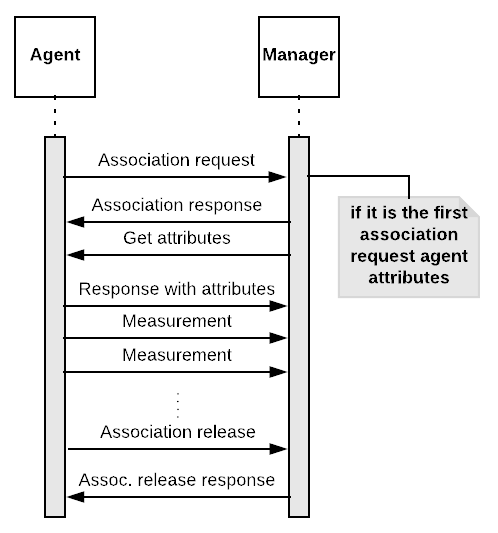
\includegraphics[scale=0.35]{figures/unconfirmed.png}}
\caption{Sequence diagram of unconfirmed operation mode of an 11073 PHD application.}
\label{fig:unconfirmedMode}
\end{figure}

\subsection{Confirmed measurement event}

Now the Fig.\ref{fig:unconfirmedMode} depicts a sequence diagram of the messaging procedure corresponding to an operation of an agent with standard configuration and with confirmed measurements events.

The initial procedure is the same as explained at Section \ref{sec:UnconfirmedMeasurementEvent}. The difference is that the manager sends an acknowledgment for every measurement received. After sending a measurement data the agent shall wait three seconds. If an answer is not received in this period the agent shall send an \textit{Association abort} to the manager and transition back to the Unassociated state. If the agent still has readings to send a new association must be done. This and others errors conditions is explained in \cite{b1}.

To avoid many associations right after a non-received ACK we implemented a stop-and-wait retransmission system in the application layer. This save the unnecessary exchange of several control packets.

\begin{figure}[htbp]
\centerline{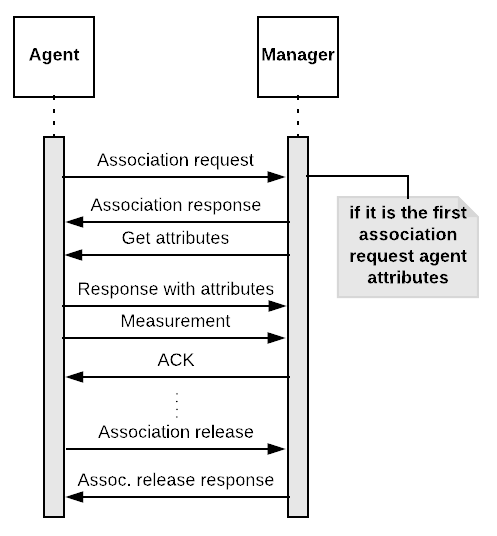
\includegraphics[scale=0.35]{figures/confirmed.png}}
\caption{Sequence diagram of confirmed operation mode of an 11073 PHD application.}
\label{fig:confirmedMode}
\end{figure}

The application also allows the user to define whether to retransmit and how many retransmission attempts. If an ACK from the manager is lost, the agent will try to retransmit the packet n times as defined by the user. When the manager finally receives the packet, it will retransmit immediately the lost ACK to the agent. The parameters implemented for retransmission are \textit{SN.node[nodeNumber].Application.retransmissionPacket} which require a boolean value and \textit{SN.node[nodeNumber].Application.maxNumOfRetransmition} that accepts an integer number. 